\documentclass{article}
\usepackage{tikz}
\usepackage{xcolor}
\definecolor{vizDefault}{HTML}{9CA3AF}
\definecolor{vizComparing}{HTML}{FFA768}
\definecolor{vizSwapping}{HTML}{E14B53}
\definecolor{vizSorted}{HTML}{5BF15D}
\definecolor{vizActive}{HTML}{629BF8}
\definecolor{vizExplored}{HTML}{7C4FDB}
\definecolor{vizUpdated}{HTML}{E0A400}
\usetikzlibrary{matrix}
\usepackage[margin=1in]{geometry}
\begin{document}
% --- Frame 0 ---
\begin{center}\LARGE\textbf{BFS}\\[6mm]\end{center}
\begin{center}
\begin{center}\textbf{Log}\\[1.75mm]\end{center}
\begin{tikzpicture}
  \filldraw[fill=white!0, draw=none] (0,0) rectangle (10cm, -0.25cm);
  \node[anchor=north, align=center, text=black] at (5cm,0) {\texttt{Initial State}};
\end{tikzpicture}
\end{center}
\noindent\rule{\linewidth}{0.3pt}
\begin{center}
\begin{center}\textbf{Graph}\\[2mm]\end{center}
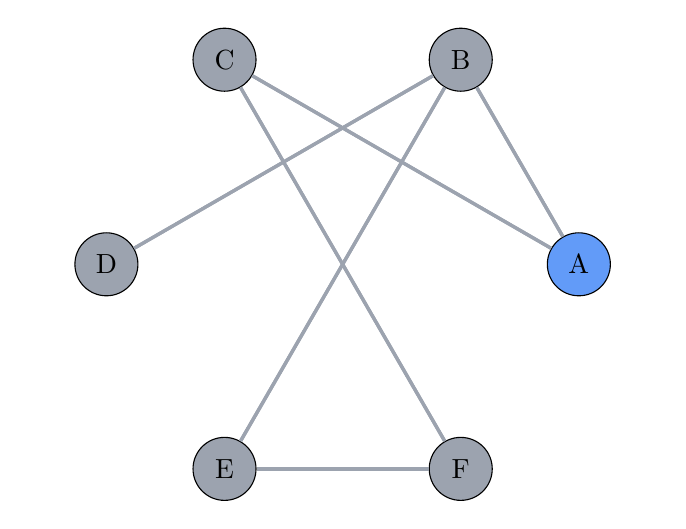
\begin{tikzpicture}
  \filldraw[fill=white!0, draw=none] (-4cm,0) rectangle (4cm, -3cm);
  \node[circle, draw, minimum size=8mm, fill=vizActive] (A) at (0.0:3cm) {A};
  \node[circle, draw, minimum size=8mm, fill=vizDefault] (B) at (60.0:3cm) {B};
  \node[circle, draw, minimum size=8mm, fill=vizDefault] (C) at (120.0:3cm) {C};
  \node[circle, draw, minimum size=8mm, fill=vizDefault] (D) at (180.0:3cm) {D};
  \node[circle, draw, minimum size=8mm, fill=vizDefault] (E) at (240.0:3cm) {E};
  \node[circle, draw, minimum size=8mm, fill=vizDefault] (F) at (300.0:3cm) {F};
  \draw[vizDefault, line width=1.2pt] (A) -- (B);
  \draw[vizDefault, line width=1.2pt] (A) -- (C);
  \draw[vizDefault, line width=1.2pt] (B) -- (A);
  \draw[vizDefault, line width=1.2pt] (B) -- (D);
  \draw[vizDefault, line width=1.2pt] (B) -- (E);
  \draw[vizDefault, line width=1.2pt] (C) -- (A);
  \draw[vizDefault, line width=1.2pt] (C) -- (F);
  \draw[vizDefault, line width=1.2pt] (D) -- (B);
  \draw[vizDefault, line width=1.2pt] (E) -- (B);
  \draw[vizDefault, line width=1.2pt] (E) -- (F);
  \draw[vizDefault, line width=1.2pt] (F) -- (C);
  \draw[vizDefault, line width=1.2pt] (F) -- (E);
\end{tikzpicture}
\end{center}
\noindent\rule{\linewidth}{0.3pt}
\begin{center}
\begin{center}\textbf{Queue}\\[1.75mm]\end{center}
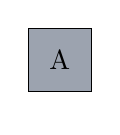
\begin{tikzpicture}
  \filldraw[fill=white!0, draw=none] (0cm,0cm) rectangle (0.8cm, -1cm);
  \filldraw[fill=vizDefault] (0cm,-0.8cm) rectangle (0.8cm,0cm);
  \node at (0.4cm,-0.4cm) {A};
\end{tikzpicture}
\end{center}
\newpage
% --- Frame 1 ---
\begin{center}\LARGE\textbf{BFS}\\[6mm]\end{center}
\begin{center}
\begin{center}\textbf{Log}\\[1.75mm]\end{center}

\begin{tikzpicture}
  \filldraw[fill=white!0, draw=none] (0,0) rectangle (10cm, -0.25cm);
  \node[anchor=north, align=center, text=black] at (5cm,0) {\texttt{Taking the first node from the queue.}};
\end{tikzpicture}
\end{center}
\noindent\rule{\linewidth}{0.3pt}
\begin{center}
\begin{center}\textbf{Graph}\\[2mm]\end{center}
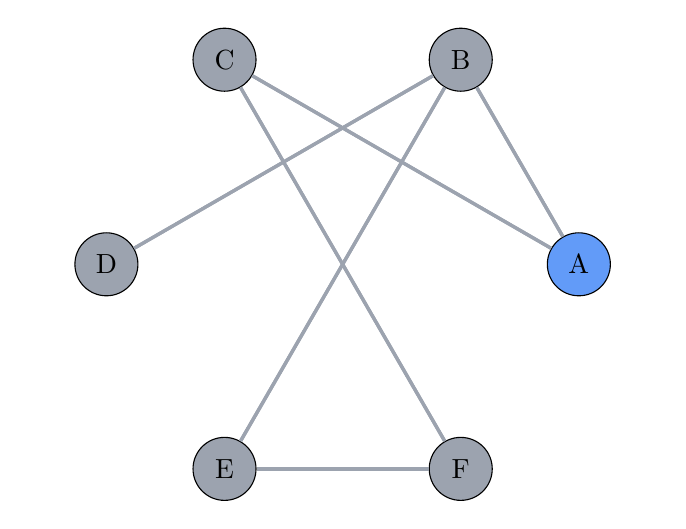
\begin{tikzpicture}
  \filldraw[fill=white!0, draw=none] (-4cm,0) rectangle (4cm, -3cm);
  \node[circle, draw, minimum size=8mm, fill=vizActive] (A) at (0.0:3cm) {A};
  \node[circle, draw, minimum size=8mm, fill=vizDefault] (B) at (60.0:3cm) {B};
  \node[circle, draw, minimum size=8mm, fill=vizDefault] (C) at (120.0:3cm) {C};
  \node[circle, draw, minimum size=8mm, fill=vizDefault] (D) at (180.0:3cm) {D};
  \node[circle, draw, minimum size=8mm, fill=vizDefault] (E) at (240.0:3cm) {E};
  \node[circle, draw, minimum size=8mm, fill=vizDefault] (F) at (300.0:3cm) {F};
  \draw[vizDefault, line width=1.2pt] (A) -- (B);
  \draw[vizDefault, line width=1.2pt] (A) -- (C);
  \draw[vizDefault, line width=1.2pt] (B) -- (A);
  \draw[vizDefault, line width=1.2pt] (B) -- (D);
  \draw[vizDefault, line width=1.2pt] (B) -- (E);
  \draw[vizDefault, line width=1.2pt] (C) -- (A);
  \draw[vizDefault, line width=1.2pt] (C) -- (F);
  \draw[vizDefault, line width=1.2pt] (D) -- (B);
  \draw[vizDefault, line width=1.2pt] (E) -- (B);
  \draw[vizDefault, line width=1.2pt] (E) -- (F);
  \draw[vizDefault, line width=1.2pt] (F) -- (C);
  \draw[vizDefault, line width=1.2pt] (F) -- (E);
\end{tikzpicture}
\end{center}
\noindent\rule{\linewidth}{0.3pt}
\begin{center}
\begin{center}\textbf{Queue}\\[1.75mm]\end{center}

\begin{tikzpicture}
  \filldraw[fill=white!0, draw=none] (0cm,0cm) rectangle (0.8cm, -1cm);
  \filldraw[fill=vizSwapping] (0cm,-0.8cm) rectangle (0.8cm,0cm);
  \node at (0.4cm,-0.4cm) {A};
\end{tikzpicture}
\end{center}
\newpage
% --- Frame 2 ---
\begin{center}\LARGE\textbf{BFS}\\[6mm]\end{center}
\begin{center}
\begin{center}\textbf{Log}\\[1.75mm]\end{center}

\begin{tikzpicture}
  \filldraw[fill=white!0, draw=none] (0,0) rectangle (10cm, -0.25cm);
  \node[anchor=north, align=center, text=black] at (5cm,0) {\texttt{Node A has not been visited yet — marking it visited.}};
\end{tikzpicture}
\end{center}
\noindent\rule{\linewidth}{0.3pt}
\begin{center}
\begin{center}\textbf{Graph}\\[2mm]\end{center}
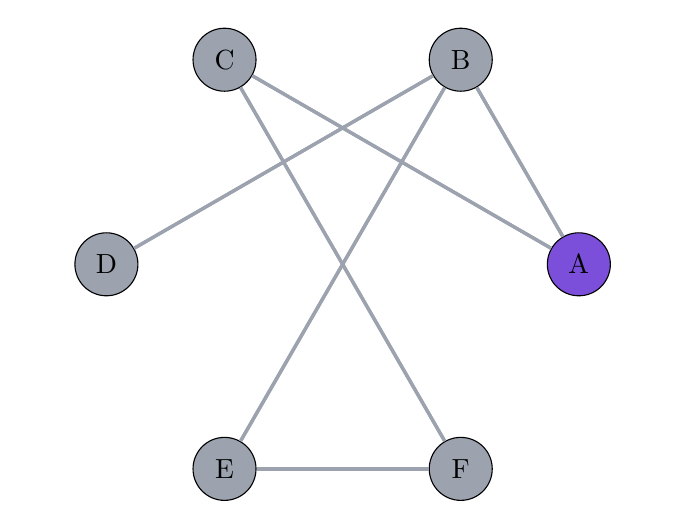
\begin{tikzpicture}
  \filldraw[fill=white!0, draw=none] (-4cm,0) rectangle (4cm, -3cm);
  \node[circle, draw, minimum size=8mm, fill=vizExplored] (A) at (0.0:3cm) {A};
  \node[circle, draw, minimum size=8mm, fill=vizDefault] (B) at (60.0:3cm) {B};
  \node[circle, draw, minimum size=8mm, fill=vizDefault] (C) at (120.0:3cm) {C};
  \node[circle, draw, minimum size=8mm, fill=vizDefault] (D) at (180.0:3cm) {D};
  \node[circle, draw, minimum size=8mm, fill=vizDefault] (E) at (240.0:3cm) {E};
  \node[circle, draw, minimum size=8mm, fill=vizDefault] (F) at (300.0:3cm) {F};
  \draw[vizDefault, line width=1.2pt] (A) -- (B);
  \draw[vizDefault, line width=1.2pt] (A) -- (C);
  \draw[vizDefault, line width=1.2pt] (B) -- (A);
  \draw[vizDefault, line width=1.2pt] (B) -- (D);
  \draw[vizDefault, line width=1.2pt] (B) -- (E);
  \draw[vizDefault, line width=1.2pt] (C) -- (A);
  \draw[vizDefault, line width=1.2pt] (C) -- (F);
  \draw[vizDefault, line width=1.2pt] (D) -- (B);
  \draw[vizDefault, line width=1.2pt] (E) -- (B);
  \draw[vizDefault, line width=1.2pt] (E) -- (F);
  \draw[vizDefault, line width=1.2pt] (F) -- (C);
  \draw[vizDefault, line width=1.2pt] (F) -- (E);
\end{tikzpicture}
\end{center}
\noindent\rule{\linewidth}{0.3pt}
\begin{center}
\begin{center}\textbf{Queue}\\[1.75mm]\end{center}
\begin{tikzpicture}
  \filldraw[fill=white!0, draw=none] (0cm,0cm) rectangle (0cm, -1cm);
\end{tikzpicture}
\end{center}
\newpage
% --- Frame 3 ---
\begin{center}\LARGE\textbf{BFS}\\[6mm]\end{center}
\begin{center}
\begin{center}\textbf{Log}\\[1.75mm]\end{center}

\begin{tikzpicture}
  \filldraw[fill=white!0, draw=none] (0,0) rectangle (10cm, -0.25cm);
  \node[anchor=north, align=center, text=black] at (5cm,0) {\texttt{Adding A's unvisited neighbors to the queue.}};
\end{tikzpicture}
\end{center}
\noindent\rule{\linewidth}{0.3pt}
\begin{center}
\begin{center}\textbf{Graph}\\[2mm]\end{center}
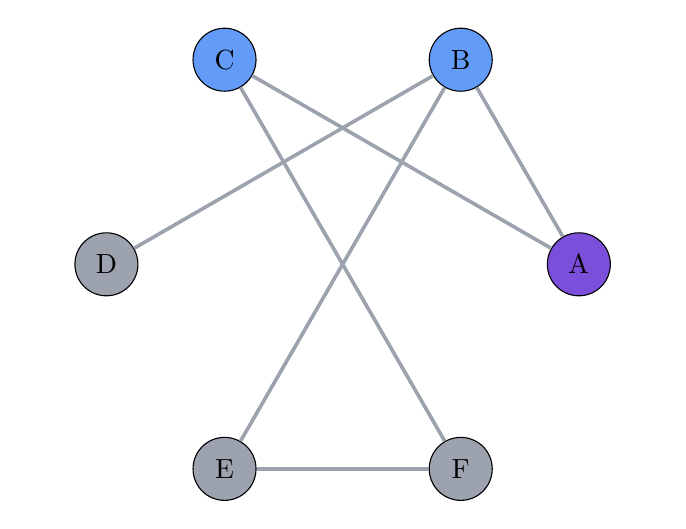
\begin{tikzpicture}
  \filldraw[fill=white!0, draw=none] (-4cm,0) rectangle (4cm, -3cm);
  \node[circle, draw, minimum size=8mm, fill=vizExplored] (A) at (0.0:3cm) {A};
  \node[circle, draw, minimum size=8mm, fill=vizActive] (B) at (60.0:3cm) {B};
  \node[circle, draw, minimum size=8mm, fill=vizActive] (C) at (120.0:3cm) {C};
  \node[circle, draw, minimum size=8mm, fill=vizDefault] (D) at (180.0:3cm) {D};
  \node[circle, draw, minimum size=8mm, fill=vizDefault] (E) at (240.0:3cm) {E};
  \node[circle, draw, minimum size=8mm, fill=vizDefault] (F) at (300.0:3cm) {F};
  \draw[vizDefault, line width=1.2pt] (A) -- (B);
  \draw[vizDefault, line width=1.2pt] (A) -- (C);
  \draw[vizDefault, line width=1.2pt] (B) -- (A);
  \draw[vizDefault, line width=1.2pt] (B) -- (D);
  \draw[vizDefault, line width=1.2pt] (B) -- (E);
  \draw[vizDefault, line width=1.2pt] (C) -- (A);
  \draw[vizDefault, line width=1.2pt] (C) -- (F);
  \draw[vizDefault, line width=1.2pt] (D) -- (B);
  \draw[vizDefault, line width=1.2pt] (E) -- (B);
  \draw[vizDefault, line width=1.2pt] (E) -- (F);
  \draw[vizDefault, line width=1.2pt] (F) -- (C);
  \draw[vizDefault, line width=1.2pt] (F) -- (E);
\end{tikzpicture}
\end{center}
\noindent\rule{\linewidth}{0.3pt}
\begin{center}
\begin{center}\textbf{Queue}\\[1.75mm]\end{center}
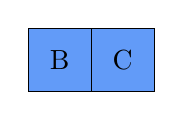
\begin{tikzpicture}
  \filldraw[fill=white!0, draw=none] (0cm,0cm) rectangle (1.6cm, -1cm);
  \filldraw[fill=vizActive] (0cm,-0.8cm) rectangle (0.8cm,0cm);
  \node at (0.4cm,-0.4cm) {B};
  \filldraw[fill=vizActive] (0.8cm,-0.8cm) rectangle (1.6cm,0cm);
  \node at (1.2000000000000002cm,-0.4cm) {C};
\end{tikzpicture}
\end{center}
\newpage
% --- Frame 4 ---
\begin{center}\LARGE\textbf{BFS}\\[6mm]\end{center}
\begin{center}
\begin{center}\textbf{Log}\\[1.75mm]\end{center}

\begin{tikzpicture}
  \filldraw[fill=white!0, draw=none] (0,0) rectangle (10cm, -0.25cm);
  \node[anchor=north, align=center, text=black] at (5cm,0) {\texttt{Adding A's unvisited neighbors to the queue.}};
\end{tikzpicture}
\end{center}
\noindent\rule{\linewidth}{0.3pt}
\begin{center}
\begin{center}\textbf{Graph}\\[2mm]\end{center}
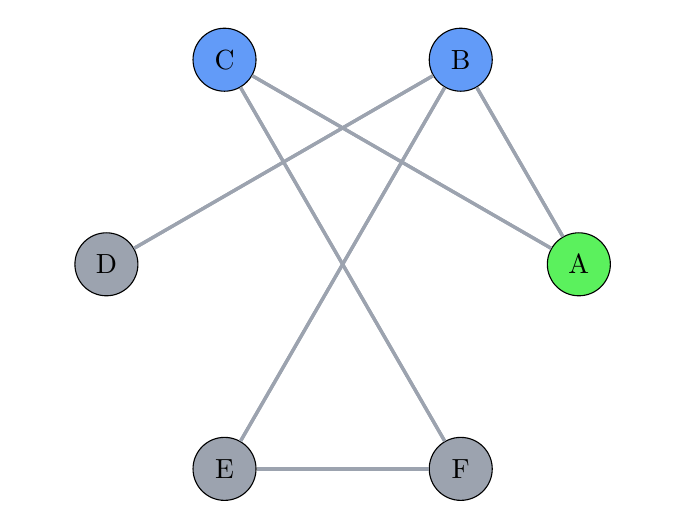
\begin{tikzpicture}
  \filldraw[fill=white!0, draw=none] (-4cm,0) rectangle (4cm, -3cm);
  \node[circle, draw, minimum size=8mm, fill=vizSorted] (A) at (0.0:3cm) {A};
  \node[circle, draw, minimum size=8mm, fill=vizActive] (B) at (60.0:3cm) {B};
  \node[circle, draw, minimum size=8mm, fill=vizActive] (C) at (120.0:3cm) {C};
  \node[circle, draw, minimum size=8mm, fill=vizDefault] (D) at (180.0:3cm) {D};
  \node[circle, draw, minimum size=8mm, fill=vizDefault] (E) at (240.0:3cm) {E};
  \node[circle, draw, minimum size=8mm, fill=vizDefault] (F) at (300.0:3cm) {F};
  \draw[vizDefault, line width=1.2pt] (A) -- (B);
  \draw[vizDefault, line width=1.2pt] (A) -- (C);
  \draw[vizDefault, line width=1.2pt] (B) -- (A);
  \draw[vizDefault, line width=1.2pt] (B) -- (D);
  \draw[vizDefault, line width=1.2pt] (B) -- (E);
  \draw[vizDefault, line width=1.2pt] (C) -- (A);
  \draw[vizDefault, line width=1.2pt] (C) -- (F);
  \draw[vizDefault, line width=1.2pt] (D) -- (B);
  \draw[vizDefault, line width=1.2pt] (E) -- (B);
  \draw[vizDefault, line width=1.2pt] (E) -- (F);
  \draw[vizDefault, line width=1.2pt] (F) -- (C);
  \draw[vizDefault, line width=1.2pt] (F) -- (E);
\end{tikzpicture}
\end{center}
\noindent\rule{\linewidth}{0.3pt}
\begin{center}
\begin{center}\textbf{Queue}\\[1.75mm]\end{center}
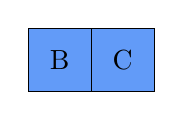
\begin{tikzpicture}
  \filldraw[fill=white!0, draw=none] (0cm,0cm) rectangle (1.6cm, -1cm);
  \filldraw[fill=vizActive] (0cm,-0.8cm) rectangle (0.8cm,0cm);
  \node at (0.4cm,-0.4cm) {B};
  \filldraw[fill=vizActive] (0.8cm,-0.8cm) rectangle (1.6cm,0cm);
  \node at (1.2000000000000002cm,-0.4cm) {C};
\end{tikzpicture}
\end{center}
\newpage
% --- Frame 5 ---
\begin{center}\LARGE\textbf{BFS}\\[6mm]\end{center}
\begin{center}
\begin{center}\textbf{Log}\\[1.75mm]\end{center}

\begin{tikzpicture}
  \filldraw[fill=white!0, draw=none] (0,0) rectangle (10cm, -0.25cm);
  \node[anchor=north, align=center, text=black] at (5cm,0) {\texttt{Taking the first node from the queue.}};
\end{tikzpicture}
\end{center}
\noindent\rule{\linewidth}{0.3pt}
\begin{center}
\begin{center}\textbf{Graph}\\[2mm]\end{center}
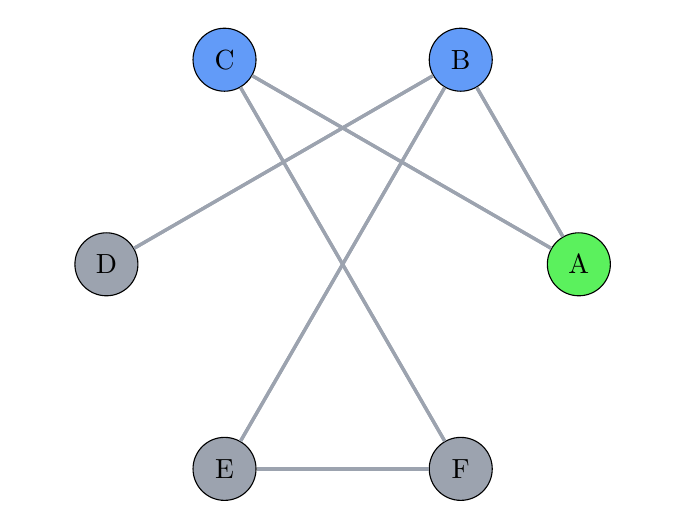
\begin{tikzpicture}
  \filldraw[fill=white!0, draw=none] (-4cm,0) rectangle (4cm, -3cm);
  \node[circle, draw, minimum size=8mm, fill=vizSorted] (A) at (0.0:3cm) {A};
  \node[circle, draw, minimum size=8mm, fill=vizActive] (B) at (60.0:3cm) {B};
  \node[circle, draw, minimum size=8mm, fill=vizActive] (C) at (120.0:3cm) {C};
  \node[circle, draw, minimum size=8mm, fill=vizDefault] (D) at (180.0:3cm) {D};
  \node[circle, draw, minimum size=8mm, fill=vizDefault] (E) at (240.0:3cm) {E};
  \node[circle, draw, minimum size=8mm, fill=vizDefault] (F) at (300.0:3cm) {F};
  \draw[vizDefault, line width=1.2pt] (A) -- (B);
  \draw[vizDefault, line width=1.2pt] (A) -- (C);
  \draw[vizDefault, line width=1.2pt] (B) -- (A);
  \draw[vizDefault, line width=1.2pt] (B) -- (D);
  \draw[vizDefault, line width=1.2pt] (B) -- (E);
  \draw[vizDefault, line width=1.2pt] (C) -- (A);
  \draw[vizDefault, line width=1.2pt] (C) -- (F);
  \draw[vizDefault, line width=1.2pt] (D) -- (B);
  \draw[vizDefault, line width=1.2pt] (E) -- (B);
  \draw[vizDefault, line width=1.2pt] (E) -- (F);
  \draw[vizDefault, line width=1.2pt] (F) -- (C);
  \draw[vizDefault, line width=1.2pt] (F) -- (E);
\end{tikzpicture}
\end{center}
\noindent\rule{\linewidth}{0.3pt}
\begin{center}
\begin{center}\textbf{Queue}\\[1.75mm]\end{center}
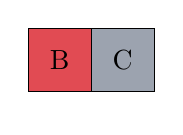
\begin{tikzpicture}
  \filldraw[fill=white!0, draw=none] (0cm,0cm) rectangle (1.6cm, -1cm);
  \filldraw[fill=vizSwapping] (0cm,-0.8cm) rectangle (0.8cm,0cm);
  \node at (0.4cm,-0.4cm) {B};
  \filldraw[fill=vizDefault] (0.8cm,-0.8cm) rectangle (1.6cm,0cm);
  \node at (1.2000000000000002cm,-0.4cm) {C};
\end{tikzpicture}
\end{center}
\newpage
% --- Frame 6 ---
\begin{center}\LARGE\textbf{BFS}\\[6mm]\end{center}
\begin{center}
\begin{center}\textbf{Log}\\[1.75mm]\end{center}

\begin{tikzpicture}
  \filldraw[fill=white!0, draw=none] (0,0) rectangle (10cm, -0.25cm);
  \node[anchor=north, align=center, text=black] at (5cm,0) {\texttt{Node B has not been visited yet — marking it visited.}};
\end{tikzpicture}
\end{center}
\noindent\rule{\linewidth}{0.3pt}
\begin{center}
\begin{center}\textbf{Graph}\\[2mm]\end{center}
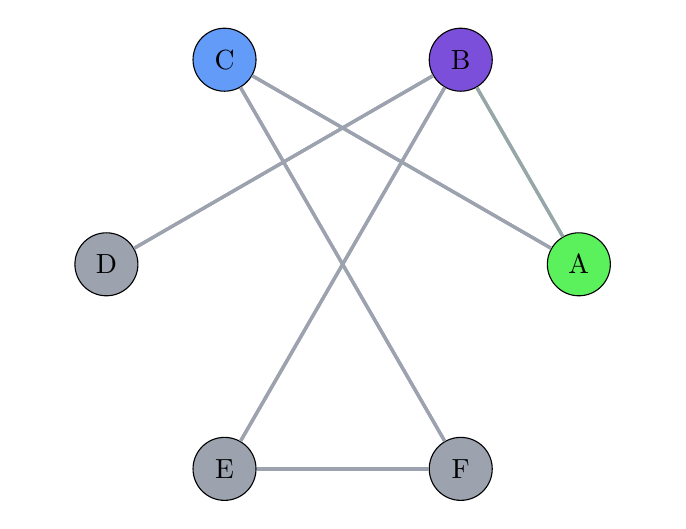
\begin{tikzpicture}
  \filldraw[fill=white!0, draw=none] (-4cm,0) rectangle (4cm, -3cm);
  \node[circle, draw, minimum size=8mm, fill=vizSorted] (A) at (0.0:3cm) {A};
  \node[circle, draw, minimum size=8mm, fill=vizExplored] (B) at (60.0:3cm) {B};
  \node[circle, draw, minimum size=8mm, fill=vizActive] (C) at (120.0:3cm) {C};
  \node[circle, draw, minimum size=8mm, fill=vizDefault] (D) at (180.0:3cm) {D};
  \node[circle, draw, minimum size=8mm, fill=vizDefault] (E) at (240.0:3cm) {E};
  \node[circle, draw, minimum size=8mm, fill=vizDefault] (F) at (300.0:3cm) {F};
  \draw[vizSorted, line width=1.2pt] (A) -- (B);
  \draw[vizDefault, line width=1.2pt] (A) -- (C);
  \draw[vizDefault, line width=1.2pt] (B) -- (A);
  \draw[vizDefault, line width=1.2pt] (B) -- (D);
  \draw[vizDefault, line width=1.2pt] (B) -- (E);
  \draw[vizDefault, line width=1.2pt] (C) -- (A);
  \draw[vizDefault, line width=1.2pt] (C) -- (F);
  \draw[vizDefault, line width=1.2pt] (D) -- (B);
  \draw[vizDefault, line width=1.2pt] (E) -- (B);
  \draw[vizDefault, line width=1.2pt] (E) -- (F);
  \draw[vizDefault, line width=1.2pt] (F) -- (C);
  \draw[vizDefault, line width=1.2pt] (F) -- (E);
\end{tikzpicture}
\end{center}
\noindent\rule{\linewidth}{0.3pt}
\begin{center}
\begin{center}\textbf{Queue}\\[1.75mm]\end{center}
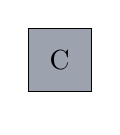
\begin{tikzpicture}
  \filldraw[fill=white!0, draw=none] (0cm,0cm) rectangle (0.8cm, -1cm);
  \filldraw[fill=vizDefault] (0cm,-0.8cm) rectangle (0.8cm,0cm);
  \node at (0.4cm,-0.4cm) {C};
\end{tikzpicture}
\end{center}
\newpage
% --- Frame 7 ---
\begin{center}\LARGE\textbf{BFS}\\[6mm]\end{center}
\begin{center}
\begin{center}\textbf{Log}\\[1.75mm]\end{center}

\begin{tikzpicture}
  \filldraw[fill=white!0, draw=none] (0,0) rectangle (10cm, -0.25cm);
  \node[anchor=north, align=center, text=black] at (5cm,0) {\texttt{Adding B's unvisited neighbors to the queue.}};
\end{tikzpicture}
\end{center}
\noindent\rule{\linewidth}{0.3pt}
\begin{center}
\begin{center}\textbf{Graph}\\[2mm]\end{center}
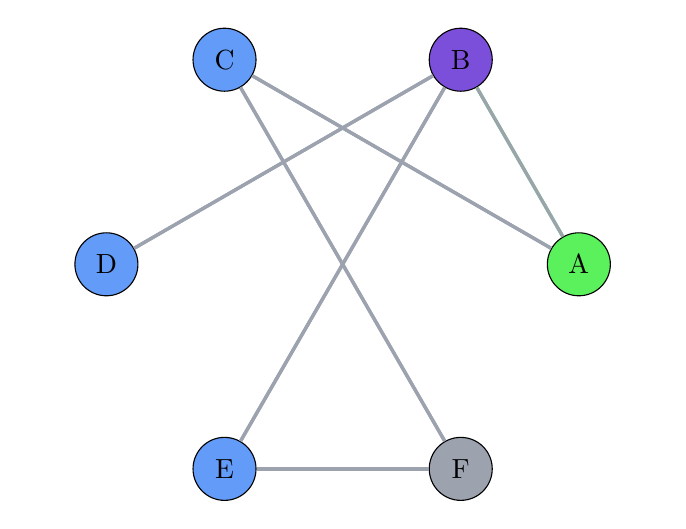
\begin{tikzpicture}
  \filldraw[fill=white!0, draw=none] (-4cm,0) rectangle (4cm, -3cm);
  \node[circle, draw, minimum size=8mm, fill=vizSorted] (A) at (0.0:3cm) {A};
  \node[circle, draw, minimum size=8mm, fill=vizExplored] (B) at (60.0:3cm) {B};
  \node[circle, draw, minimum size=8mm, fill=vizActive] (C) at (120.0:3cm) {C};
  \node[circle, draw, minimum size=8mm, fill=vizActive] (D) at (180.0:3cm) {D};
  \node[circle, draw, minimum size=8mm, fill=vizActive] (E) at (240.0:3cm) {E};
  \node[circle, draw, minimum size=8mm, fill=vizDefault] (F) at (300.0:3cm) {F};
  \draw[vizSorted, line width=1.2pt] (A) -- (B);
  \draw[vizDefault, line width=1.2pt] (A) -- (C);
  \draw[vizDefault, line width=1.2pt] (B) -- (A);
  \draw[vizDefault, line width=1.2pt] (B) -- (D);
  \draw[vizDefault, line width=1.2pt] (B) -- (E);
  \draw[vizDefault, line width=1.2pt] (C) -- (A);
  \draw[vizDefault, line width=1.2pt] (C) -- (F);
  \draw[vizDefault, line width=1.2pt] (D) -- (B);
  \draw[vizDefault, line width=1.2pt] (E) -- (B);
  \draw[vizDefault, line width=1.2pt] (E) -- (F);
  \draw[vizDefault, line width=1.2pt] (F) -- (C);
  \draw[vizDefault, line width=1.2pt] (F) -- (E);
\end{tikzpicture}
\end{center}
\noindent\rule{\linewidth}{0.3pt}
\begin{center}
\begin{center}\textbf{Queue}\\[1.75mm]\end{center}
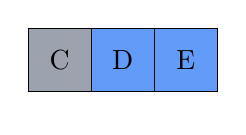
\begin{tikzpicture}
  \filldraw[fill=white!0, draw=none] (0cm,0cm) rectangle (2.4000000000000004cm, -1cm);
  \filldraw[fill=vizDefault] (0cm,-0.8cm) rectangle (0.8cm,0cm);
  \node at (0.4cm,-0.4cm) {C};
  \filldraw[fill=vizActive] (0.8cm,-0.8cm) rectangle (1.6cm,0cm);
  \node at (1.2000000000000002cm,-0.4cm) {D};
  \filldraw[fill=vizActive] (1.6cm,-0.8cm) rectangle (2.4000000000000004cm,0cm);
  \node at (2cm,-0.4cm) {E};
\end{tikzpicture}
\end{center}
\newpage
% --- Frame 8 ---
\begin{center}\LARGE\textbf{BFS}\\[6mm]\end{center}
\begin{center}
\begin{center}\textbf{Log}\\[1.75mm]\end{center}

\begin{tikzpicture}
  \filldraw[fill=white!0, draw=none] (0,0) rectangle (10cm, -0.25cm);
  \node[anchor=north, align=center, text=black] at (5cm,0) {\texttt{Adding B's unvisited neighbors to the queue.}};
\end{tikzpicture}
\end{center}
\noindent\rule{\linewidth}{0.3pt}
\begin{center}
\begin{center}\textbf{Graph}\\[2mm]\end{center}
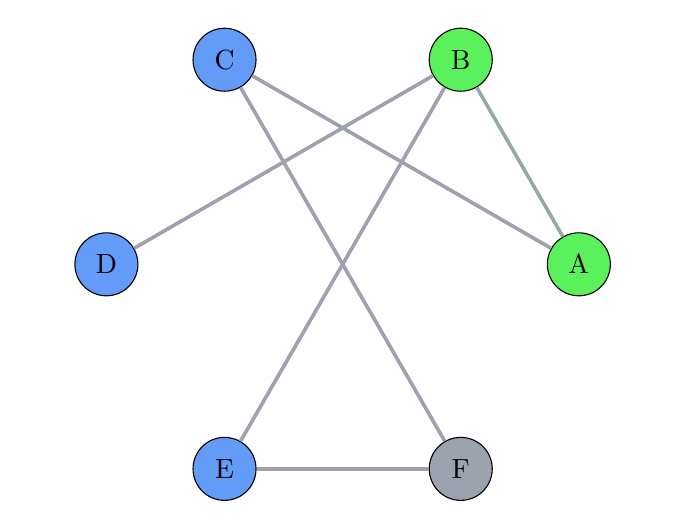
\begin{tikzpicture}
  \filldraw[fill=white!0, draw=none] (-4cm,0) rectangle (4cm, -3cm);
  \node[circle, draw, minimum size=8mm, fill=vizSorted] (A) at (0.0:3cm) {A};
  \node[circle, draw, minimum size=8mm, fill=vizSorted] (B) at (60.0:3cm) {B};
  \node[circle, draw, minimum size=8mm, fill=vizActive] (C) at (120.0:3cm) {C};
  \node[circle, draw, minimum size=8mm, fill=vizActive] (D) at (180.0:3cm) {D};
  \node[circle, draw, minimum size=8mm, fill=vizActive] (E) at (240.0:3cm) {E};
  \node[circle, draw, minimum size=8mm, fill=vizDefault] (F) at (300.0:3cm) {F};
  \draw[vizSorted, line width=1.2pt] (A) -- (B);
  \draw[vizDefault, line width=1.2pt] (A) -- (C);
  \draw[vizDefault, line width=1.2pt] (B) -- (A);
  \draw[vizDefault, line width=1.2pt] (B) -- (D);
  \draw[vizDefault, line width=1.2pt] (B) -- (E);
  \draw[vizDefault, line width=1.2pt] (C) -- (A);
  \draw[vizDefault, line width=1.2pt] (C) -- (F);
  \draw[vizDefault, line width=1.2pt] (D) -- (B);
  \draw[vizDefault, line width=1.2pt] (E) -- (B);
  \draw[vizDefault, line width=1.2pt] (E) -- (F);
  \draw[vizDefault, line width=1.2pt] (F) -- (C);
  \draw[vizDefault, line width=1.2pt] (F) -- (E);
\end{tikzpicture}
\end{center}
\noindent\rule{\linewidth}{0.3pt}
\begin{center}
\begin{center}\textbf{Queue}\\[1.75mm]\end{center}
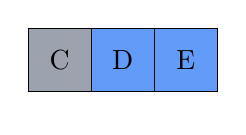
\begin{tikzpicture}
  \filldraw[fill=white!0, draw=none] (0cm,0cm) rectangle (2.4000000000000004cm, -1cm);
  \filldraw[fill=vizDefault] (0cm,-0.8cm) rectangle (0.8cm,0cm);
  \node at (0.4cm,-0.4cm) {C};
  \filldraw[fill=vizActive] (0.8cm,-0.8cm) rectangle (1.6cm,0cm);
  \node at (1.2000000000000002cm,-0.4cm) {D};
  \filldraw[fill=vizActive] (1.6cm,-0.8cm) rectangle (2.4000000000000004cm,0cm);
  \node at (2cm,-0.4cm) {E};
\end{tikzpicture}
\end{center}
\newpage
% --- Frame 9 ---
\begin{center}\LARGE\textbf{BFS}\\[6mm]\end{center}
\begin{center}
\begin{center}\textbf{Log}\\[1.75mm]\end{center}

\begin{tikzpicture}
  \filldraw[fill=white!0, draw=none] (0,0) rectangle (10cm, -0.25cm);
  \node[anchor=north, align=center, text=black] at (5cm,0) {\texttt{Taking the first node from the queue.}};
\end{tikzpicture}
\end{center}
\noindent\rule{\linewidth}{0.3pt}
\begin{center}
\begin{center}\textbf{Graph}\\[2mm]\end{center}
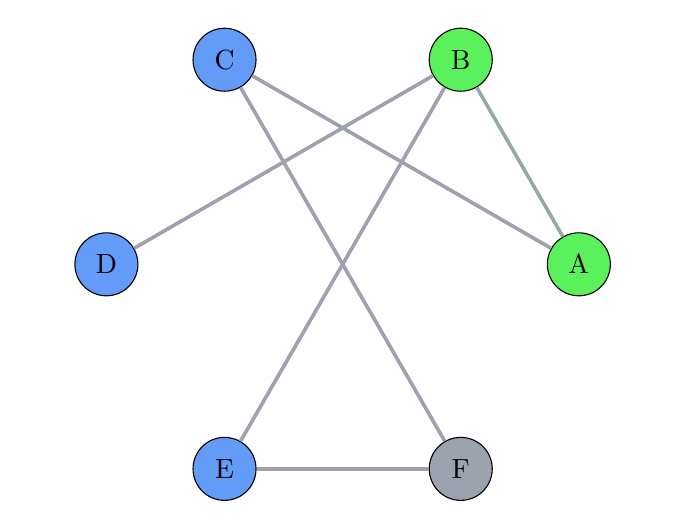
\begin{tikzpicture}
  \filldraw[fill=white!0, draw=none] (-4cm,0) rectangle (4cm, -3cm);
  \node[circle, draw, minimum size=8mm, fill=vizSorted] (A) at (0.0:3cm) {A};
  \node[circle, draw, minimum size=8mm, fill=vizSorted] (B) at (60.0:3cm) {B};
  \node[circle, draw, minimum size=8mm, fill=vizActive] (C) at (120.0:3cm) {C};
  \node[circle, draw, minimum size=8mm, fill=vizActive] (D) at (180.0:3cm) {D};
  \node[circle, draw, minimum size=8mm, fill=vizActive] (E) at (240.0:3cm) {E};
  \node[circle, draw, minimum size=8mm, fill=vizDefault] (F) at (300.0:3cm) {F};
  \draw[vizSorted, line width=1.2pt] (A) -- (B);
  \draw[vizDefault, line width=1.2pt] (A) -- (C);
  \draw[vizDefault, line width=1.2pt] (B) -- (A);
  \draw[vizDefault, line width=1.2pt] (B) -- (D);
  \draw[vizDefault, line width=1.2pt] (B) -- (E);
  \draw[vizDefault, line width=1.2pt] (C) -- (A);
  \draw[vizDefault, line width=1.2pt] (C) -- (F);
  \draw[vizDefault, line width=1.2pt] (D) -- (B);
  \draw[vizDefault, line width=1.2pt] (E) -- (B);
  \draw[vizDefault, line width=1.2pt] (E) -- (F);
  \draw[vizDefault, line width=1.2pt] (F) -- (C);
  \draw[vizDefault, line width=1.2pt] (F) -- (E);
\end{tikzpicture}
\end{center}
\noindent\rule{\linewidth}{0.3pt}
\begin{center}
\begin{center}\textbf{Queue}\\[1.75mm]\end{center}
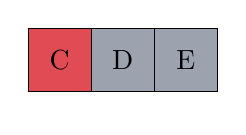
\begin{tikzpicture}
  \filldraw[fill=white!0, draw=none] (0cm,0cm) rectangle (2.4000000000000004cm, -1cm);
  \filldraw[fill=vizSwapping] (0cm,-0.8cm) rectangle (0.8cm,0cm);
  \node at (0.4cm,-0.4cm) {C};
  \filldraw[fill=vizDefault] (0.8cm,-0.8cm) rectangle (1.6cm,0cm);
  \node at (1.2000000000000002cm,-0.4cm) {D};
  \filldraw[fill=vizDefault] (1.6cm,-0.8cm) rectangle (2.4000000000000004cm,0cm);
  \node at (2cm,-0.4cm) {E};
\end{tikzpicture}
\end{center}
\newpage
% --- Frame 10 ---
\begin{center}\LARGE\textbf{BFS}\\[6mm]\end{center}
\begin{center}
\begin{center}\textbf{Log}\\[1.75mm]\end{center}

\begin{tikzpicture}
  \filldraw[fill=white!0, draw=none] (0,0) rectangle (10cm, -0.25cm);
  \node[anchor=north, align=center, text=black] at (5cm,0) {\texttt{Node C has not been visited yet — marking it visited.}};
\end{tikzpicture}
\end{center}
\noindent\rule{\linewidth}{0.3pt}
\begin{center}
\begin{center}\textbf{Graph}\\[2mm]\end{center}
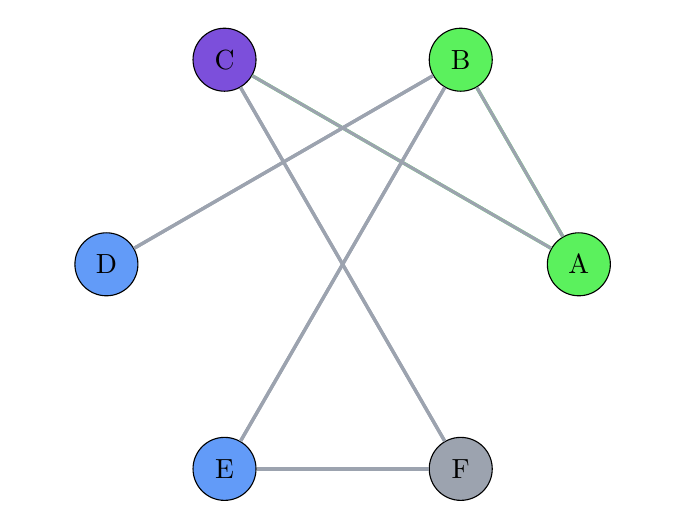
\begin{tikzpicture}
  \filldraw[fill=white!0, draw=none] (-4cm,0) rectangle (4cm, -3cm);
  \node[circle, draw, minimum size=8mm, fill=vizSorted] (A) at (0.0:3cm) {A};
  \node[circle, draw, minimum size=8mm, fill=vizSorted] (B) at (60.0:3cm) {B};
  \node[circle, draw, minimum size=8mm, fill=vizExplored] (C) at (120.0:3cm) {C};
  \node[circle, draw, minimum size=8mm, fill=vizActive] (D) at (180.0:3cm) {D};
  \node[circle, draw, minimum size=8mm, fill=vizActive] (E) at (240.0:3cm) {E};
  \node[circle, draw, minimum size=8mm, fill=vizDefault] (F) at (300.0:3cm) {F};
  \draw[vizSorted, line width=1.2pt] (A) -- (B);
  \draw[vizSorted, line width=1.2pt] (A) -- (C);
  \draw[vizDefault, line width=1.2pt] (B) -- (A);
  \draw[vizDefault, line width=1.2pt] (B) -- (D);
  \draw[vizDefault, line width=1.2pt] (B) -- (E);
  \draw[vizDefault, line width=1.2pt] (C) -- (A);
  \draw[vizDefault, line width=1.2pt] (C) -- (F);
  \draw[vizDefault, line width=1.2pt] (D) -- (B);
  \draw[vizDefault, line width=1.2pt] (E) -- (B);
  \draw[vizDefault, line width=1.2pt] (E) -- (F);
  \draw[vizDefault, line width=1.2pt] (F) -- (C);
  \draw[vizDefault, line width=1.2pt] (F) -- (E);
\end{tikzpicture}
\end{center}
\noindent\rule{\linewidth}{0.3pt}
\begin{center}
\begin{center}\textbf{Queue}\\[1.75mm]\end{center}
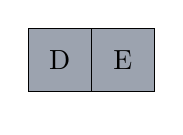
\begin{tikzpicture}
  \filldraw[fill=white!0, draw=none] (0cm,0cm) rectangle (1.6cm, -1cm);
  \filldraw[fill=vizDefault] (0cm,-0.8cm) rectangle (0.8cm,0cm);
  \node at (0.4cm,-0.4cm) {D};
  \filldraw[fill=vizDefault] (0.8cm,-0.8cm) rectangle (1.6cm,0cm);
  \node at (1.2000000000000002cm,-0.4cm) {E};
\end{tikzpicture}
\end{center}
\newpage
% --- Frame 11 ---
\begin{center}\LARGE\textbf{BFS}\\[6mm]\end{center}
\begin{center}
\begin{center}\textbf{Log}\\[1.75mm]\end{center}

\begin{tikzpicture}
  \filldraw[fill=white!0, draw=none] (0,0) rectangle (10cm, -0.25cm);
  \node[anchor=north, align=center, text=black] at (5cm,0) {\texttt{Adding C's unvisited neighbors to the queue.}};
\end{tikzpicture}
\end{center}
\noindent\rule{\linewidth}{0.3pt}
\begin{center}
\begin{center}\textbf{Graph}\\[2mm]\end{center}
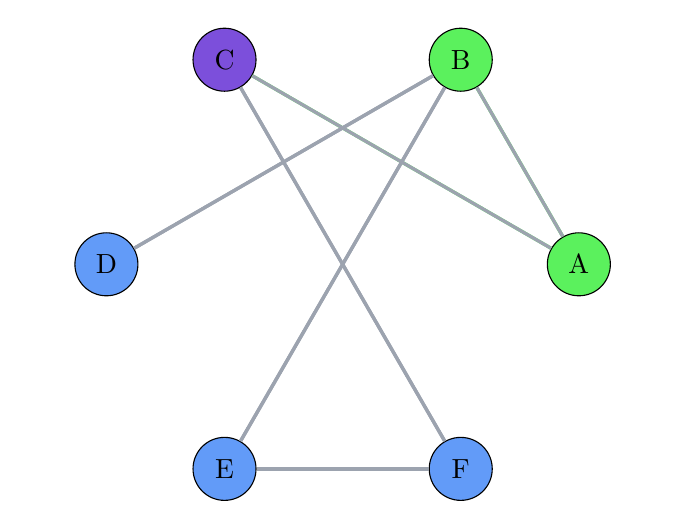
\begin{tikzpicture}
  \filldraw[fill=white!0, draw=none] (-4cm,0) rectangle (4cm, -3cm);
  \node[circle, draw, minimum size=8mm, fill=vizSorted] (A) at (0.0:3cm) {A};
  \node[circle, draw, minimum size=8mm, fill=vizSorted] (B) at (60.0:3cm) {B};
  \node[circle, draw, minimum size=8mm, fill=vizExplored] (C) at (120.0:3cm) {C};
  \node[circle, draw, minimum size=8mm, fill=vizActive] (D) at (180.0:3cm) {D};
  \node[circle, draw, minimum size=8mm, fill=vizActive] (E) at (240.0:3cm) {E};
  \node[circle, draw, minimum size=8mm, fill=vizActive] (F) at (300.0:3cm) {F};
  \draw[vizSorted, line width=1.2pt] (A) -- (B);
  \draw[vizSorted, line width=1.2pt] (A) -- (C);
  \draw[vizDefault, line width=1.2pt] (B) -- (A);
  \draw[vizDefault, line width=1.2pt] (B) -- (D);
  \draw[vizDefault, line width=1.2pt] (B) -- (E);
  \draw[vizDefault, line width=1.2pt] (C) -- (A);
  \draw[vizDefault, line width=1.2pt] (C) -- (F);
  \draw[vizDefault, line width=1.2pt] (D) -- (B);
  \draw[vizDefault, line width=1.2pt] (E) -- (B);
  \draw[vizDefault, line width=1.2pt] (E) -- (F);
  \draw[vizDefault, line width=1.2pt] (F) -- (C);
  \draw[vizDefault, line width=1.2pt] (F) -- (E);
\end{tikzpicture}
\end{center}
\noindent\rule{\linewidth}{0.3pt}
\begin{center}
\begin{center}\textbf{Queue}\\[1.75mm]\end{center}
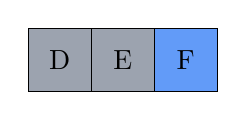
\begin{tikzpicture}
  \filldraw[fill=white!0, draw=none] (0cm,0cm) rectangle (2.4000000000000004cm, -1cm);
  \filldraw[fill=vizDefault] (0cm,-0.8cm) rectangle (0.8cm,0cm);
  \node at (0.4cm,-0.4cm) {D};
  \filldraw[fill=vizDefault] (0.8cm,-0.8cm) rectangle (1.6cm,0cm);
  \node at (1.2000000000000002cm,-0.4cm) {E};
  \filldraw[fill=vizActive] (1.6cm,-0.8cm) rectangle (2.4000000000000004cm,0cm);
  \node at (2cm,-0.4cm) {F};
\end{tikzpicture}
\end{center}
\newpage
% --- Frame 12 ---
\begin{center}\LARGE\textbf{BFS}\\[6mm]\end{center}
\begin{center}
\begin{center}\textbf{Log}\\[1.75mm]\end{center}

\begin{tikzpicture}
  \filldraw[fill=white!0, draw=none] (0,0) rectangle (10cm, -0.25cm);
  \node[anchor=north, align=center, text=black] at (5cm,0) {\texttt{Adding C's unvisited neighbors to the queue.}};
\end{tikzpicture}
\end{center}
\noindent\rule{\linewidth}{0.3pt}
\begin{center}
\begin{center}\textbf{Graph}\\[2mm]\end{center}
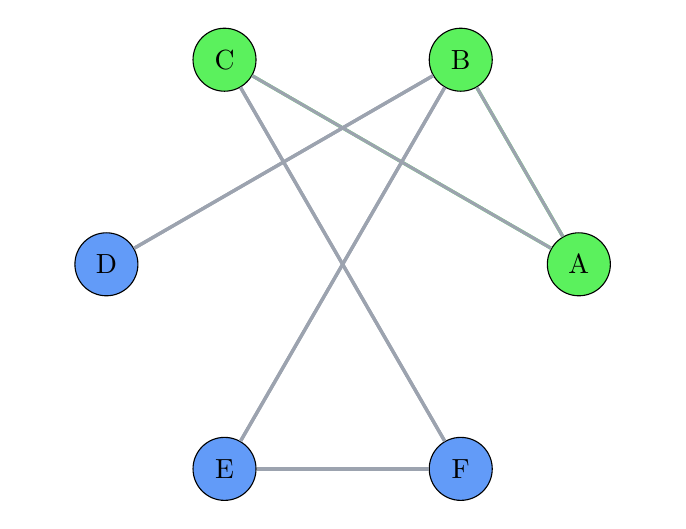
\begin{tikzpicture}
  \filldraw[fill=white!0, draw=none] (-4cm,0) rectangle (4cm, -3cm);
  \node[circle, draw, minimum size=8mm, fill=vizSorted] (A) at (0.0:3cm) {A};
  \node[circle, draw, minimum size=8mm, fill=vizSorted] (B) at (60.0:3cm) {B};
  \node[circle, draw, minimum size=8mm, fill=vizSorted] (C) at (120.0:3cm) {C};
  \node[circle, draw, minimum size=8mm, fill=vizActive] (D) at (180.0:3cm) {D};
  \node[circle, draw, minimum size=8mm, fill=vizActive] (E) at (240.0:3cm) {E};
  \node[circle, draw, minimum size=8mm, fill=vizActive] (F) at (300.0:3cm) {F};
  \draw[vizSorted, line width=1.2pt] (A) -- (B);
  \draw[vizSorted, line width=1.2pt] (A) -- (C);
  \draw[vizDefault, line width=1.2pt] (B) -- (A);
  \draw[vizDefault, line width=1.2pt] (B) -- (D);
  \draw[vizDefault, line width=1.2pt] (B) -- (E);
  \draw[vizDefault, line width=1.2pt] (C) -- (A);
  \draw[vizDefault, line width=1.2pt] (C) -- (F);
  \draw[vizDefault, line width=1.2pt] (D) -- (B);
  \draw[vizDefault, line width=1.2pt] (E) -- (B);
  \draw[vizDefault, line width=1.2pt] (E) -- (F);
  \draw[vizDefault, line width=1.2pt] (F) -- (C);
  \draw[vizDefault, line width=1.2pt] (F) -- (E);
\end{tikzpicture}
\end{center}
\noindent\rule{\linewidth}{0.3pt}
\begin{center}
\begin{center}\textbf{Queue}\\[1.75mm]\end{center}
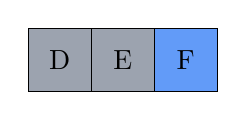
\begin{tikzpicture}
  \filldraw[fill=white!0, draw=none] (0cm,0cm) rectangle (2.4000000000000004cm, -1cm);
  \filldraw[fill=vizDefault] (0cm,-0.8cm) rectangle (0.8cm,0cm);
  \node at (0.4cm,-0.4cm) {D};
  \filldraw[fill=vizDefault] (0.8cm,-0.8cm) rectangle (1.6cm,0cm);
  \node at (1.2000000000000002cm,-0.4cm) {E};
  \filldraw[fill=vizActive] (1.6cm,-0.8cm) rectangle (2.4000000000000004cm,0cm);
  \node at (2cm,-0.4cm) {F};
\end{tikzpicture}
\end{center}
\newpage
% --- Frame 13 ---
\begin{center}\LARGE\textbf{BFS}\\[6mm]\end{center}
\begin{center}
\begin{center}\textbf{Log}\\[1.75mm]\end{center}

\begin{tikzpicture}
  \filldraw[fill=white!0, draw=none] (0,0) rectangle (10cm, -0.25cm);
  \node[anchor=north, align=center, text=black] at (5cm,0) {\texttt{Taking the first node from the queue.}};
\end{tikzpicture}
\end{center}
\noindent\rule{\linewidth}{0.3pt}
\begin{center}
\begin{center}\textbf{Graph}\\[2mm]\end{center}
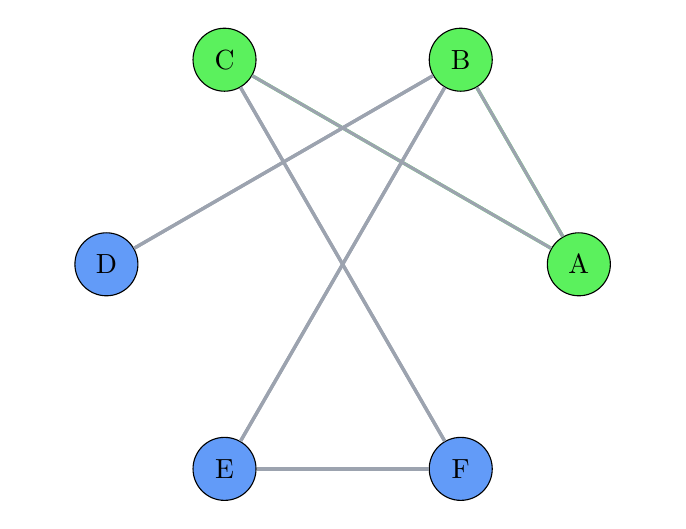
\begin{tikzpicture}
  \filldraw[fill=white!0, draw=none] (-4cm,0) rectangle (4cm, -3cm);
  \node[circle, draw, minimum size=8mm, fill=vizSorted] (A) at (0.0:3cm) {A};
  \node[circle, draw, minimum size=8mm, fill=vizSorted] (B) at (60.0:3cm) {B};
  \node[circle, draw, minimum size=8mm, fill=vizSorted] (C) at (120.0:3cm) {C};
  \node[circle, draw, minimum size=8mm, fill=vizActive] (D) at (180.0:3cm) {D};
  \node[circle, draw, minimum size=8mm, fill=vizActive] (E) at (240.0:3cm) {E};
  \node[circle, draw, minimum size=8mm, fill=vizActive] (F) at (300.0:3cm) {F};
  \draw[vizSorted, line width=1.2pt] (A) -- (B);
  \draw[vizSorted, line width=1.2pt] (A) -- (C);
  \draw[vizDefault, line width=1.2pt] (B) -- (A);
  \draw[vizDefault, line width=1.2pt] (B) -- (D);
  \draw[vizDefault, line width=1.2pt] (B) -- (E);
  \draw[vizDefault, line width=1.2pt] (C) -- (A);
  \draw[vizDefault, line width=1.2pt] (C) -- (F);
  \draw[vizDefault, line width=1.2pt] (D) -- (B);
  \draw[vizDefault, line width=1.2pt] (E) -- (B);
  \draw[vizDefault, line width=1.2pt] (E) -- (F);
  \draw[vizDefault, line width=1.2pt] (F) -- (C);
  \draw[vizDefault, line width=1.2pt] (F) -- (E);
\end{tikzpicture}
\end{center}
\noindent\rule{\linewidth}{0.3pt}
\begin{center}
\begin{center}\textbf{Queue}\\[1.75mm]\end{center}
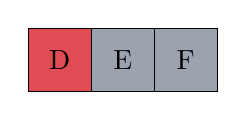
\begin{tikzpicture}
  \filldraw[fill=white!0, draw=none] (0cm,0cm) rectangle (2.4000000000000004cm, -1cm);
  \filldraw[fill=vizSwapping] (0cm,-0.8cm) rectangle (0.8cm,0cm);
  \node at (0.4cm,-0.4cm) {D};
  \filldraw[fill=vizDefault] (0.8cm,-0.8cm) rectangle (1.6cm,0cm);
  \node at (1.2000000000000002cm,-0.4cm) {E};
  \filldraw[fill=vizDefault] (1.6cm,-0.8cm) rectangle (2.4000000000000004cm,0cm);
  \node at (2cm,-0.4cm) {F};
\end{tikzpicture}
\end{center}
\newpage
% --- Frame 14 ---
\begin{center}\LARGE\textbf{BFS}\\[6mm]\end{center}
\begin{center}
\begin{center}\textbf{Log}\\[1.75mm]\end{center}

\begin{tikzpicture}
  \filldraw[fill=white!0, draw=none] (0,0) rectangle (10cm, -0.25cm);
  \node[anchor=north, align=center, text=black] at (5cm,0) {\texttt{Node D has not been visited yet — marking it visited.}};
\end{tikzpicture}
\end{center}
\noindent\rule{\linewidth}{0.3pt}
\begin{center}
\begin{center}\textbf{Graph}\\[2mm]\end{center}
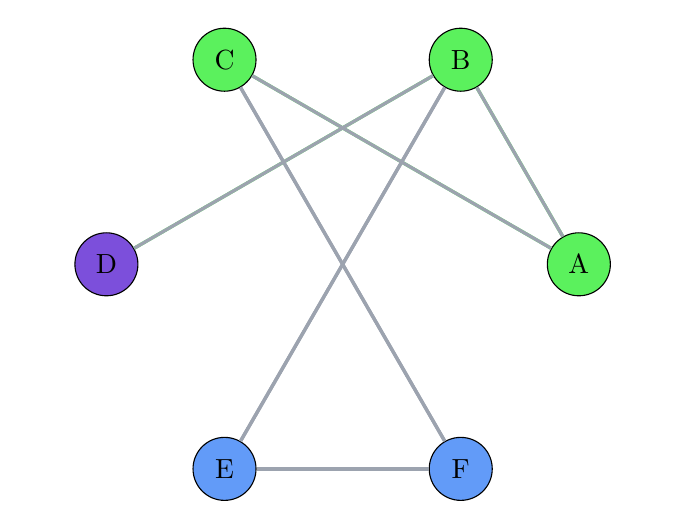
\begin{tikzpicture}
  \filldraw[fill=white!0, draw=none] (-4cm,0) rectangle (4cm, -3cm);
  \node[circle, draw, minimum size=8mm, fill=vizSorted] (A) at (0.0:3cm) {A};
  \node[circle, draw, minimum size=8mm, fill=vizSorted] (B) at (60.0:3cm) {B};
  \node[circle, draw, minimum size=8mm, fill=vizSorted] (C) at (120.0:3cm) {C};
  \node[circle, draw, minimum size=8mm, fill=vizExplored] (D) at (180.0:3cm) {D};
  \node[circle, draw, minimum size=8mm, fill=vizActive] (E) at (240.0:3cm) {E};
  \node[circle, draw, minimum size=8mm, fill=vizActive] (F) at (300.0:3cm) {F};
  \draw[vizSorted, line width=1.2pt] (A) -- (B);
  \draw[vizSorted, line width=1.2pt] (A) -- (C);
  \draw[vizDefault, line width=1.2pt] (B) -- (A);
  \draw[vizSorted, line width=1.2pt] (B) -- (D);
  \draw[vizDefault, line width=1.2pt] (B) -- (E);
  \draw[vizDefault, line width=1.2pt] (C) -- (A);
  \draw[vizDefault, line width=1.2pt] (C) -- (F);
  \draw[vizDefault, line width=1.2pt] (D) -- (B);
  \draw[vizDefault, line width=1.2pt] (E) -- (B);
  \draw[vizDefault, line width=1.2pt] (E) -- (F);
  \draw[vizDefault, line width=1.2pt] (F) -- (C);
  \draw[vizDefault, line width=1.2pt] (F) -- (E);
\end{tikzpicture}
\end{center}
\noindent\rule{\linewidth}{0.3pt}
\begin{center}
\begin{center}\textbf{Queue}\\[1.75mm]\end{center}
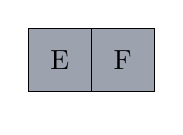
\begin{tikzpicture}
  \filldraw[fill=white!0, draw=none] (0cm,0cm) rectangle (1.6cm, -1cm);
  \filldraw[fill=vizDefault] (0cm,-0.8cm) rectangle (0.8cm,0cm);
  \node at (0.4cm,-0.4cm) {E};
  \filldraw[fill=vizDefault] (0.8cm,-0.8cm) rectangle (1.6cm,0cm);
  \node at (1.2000000000000002cm,-0.4cm) {F};
\end{tikzpicture}
\end{center}
\newpage
% --- Frame 15 ---
\begin{center}\LARGE\textbf{BFS}\\[6mm]\end{center}
\begin{center}
\begin{center}\textbf{Log}\\[1.75mm]\end{center}

\begin{tikzpicture}
  \filldraw[fill=white!0, draw=none] (0,0) rectangle (10cm, -0.25cm);
  \node[anchor=north, align=center, text=black] at (5cm,0) {\texttt{Node D has not been visited yet — marking it visited.}};
\end{tikzpicture}
\end{center}
\noindent\rule{\linewidth}{0.3pt}
\begin{center}
\begin{center}\textbf{Graph}\\[2mm]\end{center}
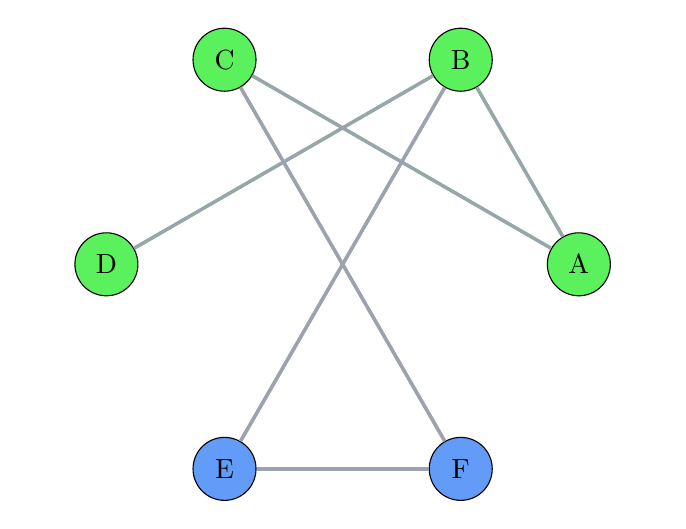
\begin{tikzpicture}
  \filldraw[fill=white!0, draw=none] (-4cm,0) rectangle (4cm, -3cm);
  \node[circle, draw, minimum size=8mm, fill=vizSorted] (A) at (0.0:3cm) {A};
  \node[circle, draw, minimum size=8mm, fill=vizSorted] (B) at (60.0:3cm) {B};
  \node[circle, draw, minimum size=8mm, fill=vizSorted] (C) at (120.0:3cm) {C};
  \node[circle, draw, minimum size=8mm, fill=vizSorted] (D) at (180.0:3cm) {D};
  \node[circle, draw, minimum size=8mm, fill=vizActive] (E) at (240.0:3cm) {E};
  \node[circle, draw, minimum size=8mm, fill=vizActive] (F) at (300.0:3cm) {F};
  \draw[vizSorted, line width=1.2pt] (A) -- (B);
  \draw[vizSorted, line width=1.2pt] (A) -- (C);
  \draw[vizDefault, line width=1.2pt] (B) -- (A);
  \draw[vizSorted, line width=1.2pt] (B) -- (D);
  \draw[vizDefault, line width=1.2pt] (B) -- (E);
  \draw[vizDefault, line width=1.2pt] (C) -- (A);
  \draw[vizDefault, line width=1.2pt] (C) -- (F);
  \draw[vizDefault, line width=1.2pt] (D) -- (B);
  \draw[vizDefault, line width=1.2pt] (E) -- (B);
  \draw[vizDefault, line width=1.2pt] (E) -- (F);
  \draw[vizDefault, line width=1.2pt] (F) -- (C);
  \draw[vizDefault, line width=1.2pt] (F) -- (E);
\end{tikzpicture}
\end{center}
\noindent\rule{\linewidth}{0.3pt}
\begin{center}
\begin{center}\textbf{Queue}\\[1.75mm]\end{center}
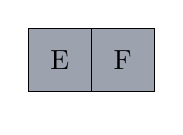
\begin{tikzpicture}
  \filldraw[fill=white!0, draw=none] (0cm,0cm) rectangle (1.6cm, -1cm);
  \filldraw[fill=vizDefault] (0cm,-0.8cm) rectangle (0.8cm,0cm);
  \node at (0.4cm,-0.4cm) {E};
  \filldraw[fill=vizDefault] (0.8cm,-0.8cm) rectangle (1.6cm,0cm);
  \node at (1.2000000000000002cm,-0.4cm) {F};
\end{tikzpicture}
\end{center}
\newpage
% --- Frame 16 ---
\begin{center}\LARGE\textbf{BFS}\\[6mm]\end{center}
\begin{center}
\begin{center}\textbf{Log}\\[1.75mm]\end{center}

\begin{tikzpicture}
  \filldraw[fill=white!0, draw=none] (0,0) rectangle (10cm, -0.25cm);
  \node[anchor=north, align=center, text=black] at (5cm,0) {\texttt{Taking the first node from the queue.}};
\end{tikzpicture}
\end{center}
\noindent\rule{\linewidth}{0.3pt}
\begin{center}
\begin{center}\textbf{Graph}\\[2mm]\end{center}
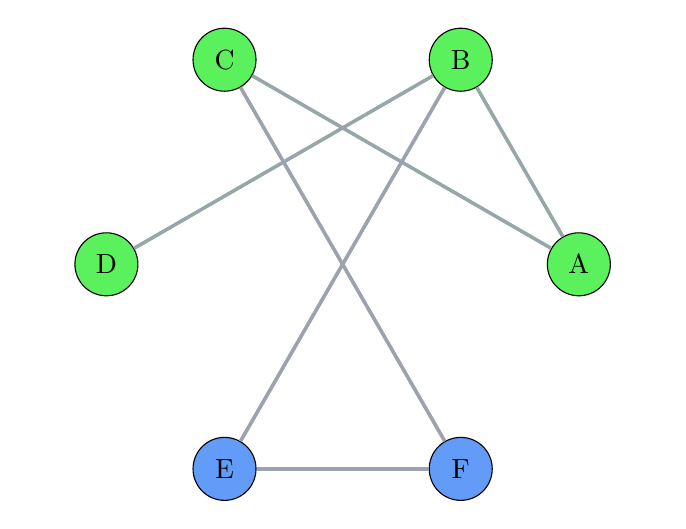
\begin{tikzpicture}
  \filldraw[fill=white!0, draw=none] (-4cm,0) rectangle (4cm, -3cm);
  \node[circle, draw, minimum size=8mm, fill=vizSorted] (A) at (0.0:3cm) {A};
  \node[circle, draw, minimum size=8mm, fill=vizSorted] (B) at (60.0:3cm) {B};
  \node[circle, draw, minimum size=8mm, fill=vizSorted] (C) at (120.0:3cm) {C};
  \node[circle, draw, minimum size=8mm, fill=vizSorted] (D) at (180.0:3cm) {D};
  \node[circle, draw, minimum size=8mm, fill=vizActive] (E) at (240.0:3cm) {E};
  \node[circle, draw, minimum size=8mm, fill=vizActive] (F) at (300.0:3cm) {F};
  \draw[vizSorted, line width=1.2pt] (A) -- (B);
  \draw[vizSorted, line width=1.2pt] (A) -- (C);
  \draw[vizDefault, line width=1.2pt] (B) -- (A);
  \draw[vizSorted, line width=1.2pt] (B) -- (D);
  \draw[vizDefault, line width=1.2pt] (B) -- (E);
  \draw[vizDefault, line width=1.2pt] (C) -- (A);
  \draw[vizDefault, line width=1.2pt] (C) -- (F);
  \draw[vizDefault, line width=1.2pt] (D) -- (B);
  \draw[vizDefault, line width=1.2pt] (E) -- (B);
  \draw[vizDefault, line width=1.2pt] (E) -- (F);
  \draw[vizDefault, line width=1.2pt] (F) -- (C);
  \draw[vizDefault, line width=1.2pt] (F) -- (E);
\end{tikzpicture}
\end{center}
\noindent\rule{\linewidth}{0.3pt}
\begin{center}
\begin{center}\textbf{Queue}\\[1.75mm]\end{center}
\begin{tikzpicture}
  \filldraw[fill=white!0, draw=none] (0cm,0cm) rectangle (1.6cm, -1cm);
  \filldraw[fill=vizSwapping] (0cm,-0.8cm) rectangle (0.8cm,0cm);
  \node at (0.4cm,-0.4cm) {E};
  \filldraw[fill=vizDefault] (0.8cm,-0.8cm) rectangle (1.6cm,0cm);
  \node at (1.2000000000000002cm,-0.4cm) {F};
\end{tikzpicture}
\end{center}
\newpage
% --- Frame 17 ---
\begin{center}\LARGE\textbf{BFS}\\[6mm]\end{center}
\begin{center}
\begin{center}\textbf{Log}\\[1.75mm]\end{center}
\begin{tikzpicture}
  \filldraw[fill=white!0, draw=none] (0,0) rectangle (10cm, -0.25cm);
  \node[anchor=north, align=center, text=black] at (5cm,0) {\texttt{Node E has not been visited yet — marking it visited.}};
\end{tikzpicture}
\end{center}
\noindent\rule{\linewidth}{0.3pt}
\begin{center}
\begin{center}\textbf{Graph}\\[2mm]\end{center}
\begin{tikzpicture}
  \filldraw[fill=white!0, draw=none] (-4cm,0) rectangle (4cm, -3cm);
  \node[circle, draw, minimum size=8mm, fill=vizSorted] (A) at (0.0:3cm) {A};
  \node[circle, draw, minimum size=8mm, fill=vizSorted] (B) at (60.0:3cm) {B};
  \node[circle, draw, minimum size=8mm, fill=vizSorted] (C) at (120.0:3cm) {C};
  \node[circle, draw, minimum size=8mm, fill=vizSorted] (D) at (180.0:3cm) {D};
  \node[circle, draw, minimum size=8mm, fill=vizExplored] (E) at (240.0:3cm) {E};
  \node[circle, draw, minimum size=8mm, fill=vizActive] (F) at (300.0:3cm) {F};
  \draw[vizSorted, line width=1.2pt] (A) -- (B);
  \draw[vizSorted, line width=1.2pt] (A) -- (C);
  \draw[vizDefault, line width=1.2pt] (B) -- (A);
  \draw[vizSorted, line width=1.2pt] (B) -- (D);
  \draw[vizSorted, line width=1.2pt] (B) -- (E);
  \draw[vizDefault, line width=1.2pt] (C) -- (A);
  \draw[vizDefault, line width=1.2pt] (C) -- (F);
  \draw[vizDefault, line width=1.2pt] (D) -- (B);
  \draw[vizDefault, line width=1.2pt] (E) -- (B);
  \draw[vizDefault, line width=1.2pt] (E) -- (F);
  \draw[vizDefault, line width=1.2pt] (F) -- (C);
  \draw[vizDefault, line width=1.2pt] (F) -- (E);
\end{tikzpicture}
\end{center}
\noindent\rule{\linewidth}{0.3pt}
\begin{center}
\begin{center}\textbf{Queue}\\[1.75mm]\end{center}
\begin{tikzpicture}
  \filldraw[fill=white!0, draw=none] (0cm,0cm) rectangle (0.8cm, -1cm);
  \filldraw[fill=vizDefault] (0cm,-0.8cm) rectangle (0.8cm,0cm);
  \node at (0.4cm,-0.4cm) {F};
\end{tikzpicture}
\end{center}
\newpage
% --- Frame 18 ---
\begin{center}\LARGE\textbf{BFS}\\[6mm]\end{center}
\begin{center}
\begin{center}\textbf{Log}\\[1.75mm]\end{center}
\begin{tikzpicture}
  \filldraw[fill=white!0, draw=none] (0,0) rectangle (10cm, -0.25cm);
  \node[anchor=north, align=center, text=black] at (5cm,0) {\texttt{Adding E's unvisited neighbors to the queue.}};
\end{tikzpicture}
\end{center}
\noindent\rule{\linewidth}{0.3pt}
\begin{center}
\begin{center}\textbf{Graph}\\[2mm]\end{center}
\begin{tikzpicture}
  \filldraw[fill=white!0, draw=none] (-4cm,0) rectangle (4cm, -3cm);
  \node[circle, draw, minimum size=8mm, fill=vizSorted] (A) at (0.0:3cm) {A};
  \node[circle, draw, minimum size=8mm, fill=vizSorted] (B) at (60.0:3cm) {B};
  \node[circle, draw, minimum size=8mm, fill=vizSorted] (C) at (120.0:3cm) {C};
  \node[circle, draw, minimum size=8mm, fill=vizSorted] (D) at (180.0:3cm) {D};
  \node[circle, draw, minimum size=8mm, fill=vizExplored] (E) at (240.0:3cm) {E};
  \node[circle, draw, minimum size=8mm, fill=vizActive] (F) at (300.0:3cm) {F};
  \draw[vizSorted, line width=1.2pt] (A) -- (B);
  \draw[vizSorted, line width=1.2pt] (A) -- (C);
  \draw[vizDefault, line width=1.2pt] (B) -- (A);
  \draw[vizSorted, line width=1.2pt] (B) -- (D);
  \draw[vizSorted, line width=1.2pt] (B) -- (E);
  \draw[vizDefault, line width=1.2pt] (C) -- (A);
  \draw[vizDefault, line width=1.2pt] (C) -- (F);
  \draw[vizDefault, line width=1.2pt] (D) -- (B);
  \draw[vizDefault, line width=1.2pt] (E) -- (B);
  \draw[vizDefault, line width=1.2pt] (E) -- (F);
  \draw[vizDefault, line width=1.2pt] (F) -- (C);
  \draw[vizDefault, line width=1.2pt] (F) -- (E);
\end{tikzpicture}
\end{center}
\noindent\rule{\linewidth}{0.3pt}
\begin{center}
\begin{center}\textbf{Queue}\\[1.75mm]\end{center}
\begin{tikzpicture}
  \filldraw[fill=white!0, draw=none] (0cm,0cm) rectangle (1.6cm, -1cm);
  \filldraw[fill=vizDefault] (0cm,-0.8cm) rectangle (0.8cm,0cm);
  \node at (0.4cm,-0.4cm) {F};
  \filldraw[fill=vizActive] (0.8cm,-0.8cm) rectangle (1.6cm,0cm);
  \node at (1.2000000000000002cm,-0.4cm) {F};
\end{tikzpicture}
\end{center}
\newpage
% --- Frame 19 ---
\begin{center}\LARGE\textbf{BFS}\\[6mm]\end{center}
\begin{center}
\begin{center}\textbf{Log}\\[1.75mm]\end{center}
\begin{tikzpicture}
  \filldraw[fill=white!0, draw=none] (0,0) rectangle (10cm, -0.25cm);
  \node[anchor=north, align=center, text=black] at (5cm,0) {\texttt{Adding E's unvisited neighbors to the queue.}};
\end{tikzpicture}
\end{center}
\noindent\rule{\linewidth}{0.3pt}
\begin{center}
\begin{center}\textbf{Graph}\\[2mm]\end{center}
\begin{tikzpicture}
  \filldraw[fill=white!0, draw=none] (-4cm,0) rectangle (4cm, -3cm);
  \node[circle, draw, minimum size=8mm, fill=vizSorted] (A) at (0.0:3cm) {A};
  \node[circle, draw, minimum size=8mm, fill=vizSorted] (B) at (60.0:3cm) {B};
  \node[circle, draw, minimum size=8mm, fill=vizSorted] (C) at (120.0:3cm) {C};
  \node[circle, draw, minimum size=8mm, fill=vizSorted] (D) at (180.0:3cm) {D};
  \node[circle, draw, minimum size=8mm, fill=vizSorted] (E) at (240.0:3cm) {E};
  \node[circle, draw, minimum size=8mm, fill=vizActive] (F) at (300.0:3cm) {F};
  \draw[vizSorted, line width=1.2pt] (A) -- (B);
  \draw[vizSorted, line width=1.2pt] (A) -- (C);
  \draw[vizDefault, line width=1.2pt] (B) -- (A);
  \draw[vizSorted, line width=1.2pt] (B) -- (D);
  \draw[vizSorted, line width=1.2pt] (B) -- (E);
  \draw[vizDefault, line width=1.2pt] (C) -- (A);
  \draw[vizDefault, line width=1.2pt] (C) -- (F);
  \draw[vizDefault, line width=1.2pt] (D) -- (B);
  \draw[vizDefault, line width=1.2pt] (E) -- (B);
  \draw[vizDefault, line width=1.2pt] (E) -- (F);
  \draw[vizDefault, line width=1.2pt] (F) -- (C);
  \draw[vizDefault, line width=1.2pt] (F) -- (E);
\end{tikzpicture}
\end{center}
\noindent\rule{\linewidth}{0.3pt}
\begin{center}
\begin{center}\textbf{Queue}\\[1.75mm]\end{center}
\begin{tikzpicture}
  \filldraw[fill=white!0, draw=none] (0cm,0cm) rectangle (1.6cm, -1cm);
  \filldraw[fill=vizDefault] (0cm,-0.8cm) rectangle (0.8cm,0cm);
  \node at (0.4cm,-0.4cm) {F};
  \filldraw[fill=vizActive] (0.8cm,-0.8cm) rectangle (1.6cm,0cm);
  \node at (1.2000000000000002cm,-0.4cm) {F};
\end{tikzpicture}
\end{center}
\newpage
% --- Frame 20 ---
\begin{center}\LARGE\textbf{BFS}\\[6mm]\end{center}
\begin{center}
\begin{center}\textbf{Log}\\[1.75mm]\end{center}
\begin{tikzpicture}
  \filldraw[fill=white!0, draw=none] (0,0) rectangle (10cm, -0.25cm);
  \node[anchor=north, align=center, text=black] at (5cm,0) {\texttt{Taking the first node from the queue.}};
\end{tikzpicture}
\end{center}
\noindent\rule{\linewidth}{0.3pt}
\begin{center}
\begin{center}\textbf{Graph}\\[2mm]\end{center}
\begin{tikzpicture}
  \filldraw[fill=white!0, draw=none] (-4cm,0) rectangle (4cm, -3cm);
  \node[circle, draw, minimum size=8mm, fill=vizSorted] (A) at (0.0:3cm) {A};
  \node[circle, draw, minimum size=8mm, fill=vizSorted] (B) at (60.0:3cm) {B};
  \node[circle, draw, minimum size=8mm, fill=vizSorted] (C) at (120.0:3cm) {C};
  \node[circle, draw, minimum size=8mm, fill=vizSorted] (D) at (180.0:3cm) {D};
  \node[circle, draw, minimum size=8mm, fill=vizSorted] (E) at (240.0:3cm) {E};
  \node[circle, draw, minimum size=8mm, fill=vizActive] (F) at (300.0:3cm) {F};
  \draw[vizSorted, line width=1.2pt] (A) -- (B);
  \draw[vizSorted, line width=1.2pt] (A) -- (C);
  \draw[vizDefault, line width=1.2pt] (B) -- (A);
  \draw[vizSorted, line width=1.2pt] (B) -- (D);
  \draw[vizSorted, line width=1.2pt] (B) -- (E);
  \draw[vizDefault, line width=1.2pt] (C) -- (A);
  \draw[vizDefault, line width=1.2pt] (C) -- (F);
  \draw[vizDefault, line width=1.2pt] (D) -- (B);
  \draw[vizDefault, line width=1.2pt] (E) -- (B);
  \draw[vizDefault, line width=1.2pt] (E) -- (F);
  \draw[vizDefault, line width=1.2pt] (F) -- (C);
  \draw[vizDefault, line width=1.2pt] (F) -- (E);
\end{tikzpicture}
\end{center}
\noindent\rule{\linewidth}{0.3pt}
\begin{center}
\begin{center}\textbf{Queue}\\[1.75mm]\end{center}
\begin{tikzpicture}
  \filldraw[fill=white!0, draw=none] (0cm,0cm) rectangle (1.6cm, -1cm);
  \filldraw[fill=vizSwapping] (0cm,-0.8cm) rectangle (0.8cm,0cm);
  \node at (0.4cm,-0.4cm) {F};
  \filldraw[fill=vizDefault] (0.8cm,-0.8cm) rectangle (1.6cm,0cm);
  \node at (1.2000000000000002cm,-0.4cm) {F};
\end{tikzpicture}
\end{center}
\newpage
% --- Frame 21 ---
\begin{center}\LARGE\textbf{BFS}\\[6mm]\end{center}
\begin{center}
\begin{center}\textbf{Log}\\[1.75mm]\end{center}
\begin{tikzpicture}
  \filldraw[fill=white!0, draw=none] (0,0) rectangle (10cm, -0.25cm);
  \node[anchor=north, align=center, text=black] at (5cm,0) {\texttt{Node F has not been visited yet — marking it visited.}};
\end{tikzpicture}
\end{center}
\noindent\rule{\linewidth}{0.3pt}
\begin{center}
\begin{center}\textbf{Graph}\\[2mm]\end{center}
\begin{tikzpicture}
  \filldraw[fill=white!0, draw=none] (-4cm,0) rectangle (4cm, -3cm);
  \node[circle, draw, minimum size=8mm, fill=vizSorted] (A) at (0.0:3cm) {A};
  \node[circle, draw, minimum size=8mm, fill=vizSorted] (B) at (60.0:3cm) {B};
  \node[circle, draw, minimum size=8mm, fill=vizSorted] (C) at (120.0:3cm) {C};
  \node[circle, draw, minimum size=8mm, fill=vizSorted] (D) at (180.0:3cm) {D};
  \node[circle, draw, minimum size=8mm, fill=vizSorted] (E) at (240.0:3cm) {E};
  \node[circle, draw, minimum size=8mm, fill=vizExplored] (F) at (300.0:3cm) {F};
  \draw[vizSorted, line width=1.2pt] (A) -- (B);
  \draw[vizSorted, line width=1.2pt] (A) -- (C);
  \draw[vizDefault, line width=1.2pt] (B) -- (A);
  \draw[vizSorted, line width=1.2pt] (B) -- (D);
  \draw[vizSorted, line width=1.2pt] (B) -- (E);
  \draw[vizDefault, line width=1.2pt] (C) -- (A);
  \draw[vizSorted, line width=1.2pt] (C) -- (F);
  \draw[vizDefault, line width=1.2pt] (D) -- (B);
  \draw[vizDefault, line width=1.2pt] (E) -- (B);
  \draw[vizDefault, line width=1.2pt] (E) -- (F);
  \draw[vizDefault, line width=1.2pt] (F) -- (C);
  \draw[vizDefault, line width=1.2pt] (F) -- (E);
\end{tikzpicture}
\end{center}
\noindent\rule{\linewidth}{0.3pt}
\begin{center}
\begin{center}\textbf{Queue}\\[1.75mm]\end{center}
\begin{tikzpicture}
  \filldraw[fill=white!0, draw=none] (0cm,0cm) rectangle (0.8cm, -1cm);
  \filldraw[fill=vizDefault] (0cm,-0.8cm) rectangle (0.8cm,0cm);
  \node at (0.4cm,-0.4cm) {F};
\end{tikzpicture}
\end{center}
\newpage
% --- Frame 22 ---
\begin{center}\LARGE\textbf{BFS}\\[6mm]\end{center}
\begin{center}
\begin{center}\textbf{Log}\\[1.75mm]\end{center}
\begin{tikzpicture}
  \filldraw[fill=white!0, draw=none] (0,0) rectangle (10cm, -0.25cm);
  \node[anchor=north, align=center, text=black] at (5cm,0) {\texttt{Node F has not been visited yet — marking it visited.}};
\end{tikzpicture}
\end{center}
\noindent\rule{\linewidth}{0.3pt}
\begin{center}
\begin{center}\textbf{Graph}\\[2mm]\end{center}
\begin{tikzpicture}
  \filldraw[fill=white!0, draw=none] (-4cm,0) rectangle (4cm, -3cm);
  \node[circle, draw, minimum size=8mm, fill=vizSorted] (A) at (0.0:3cm) {A};
  \node[circle, draw, minimum size=8mm, fill=vizSorted] (B) at (60.0:3cm) {B};
  \node[circle, draw, minimum size=8mm, fill=vizSorted] (C) at (120.0:3cm) {C};
  \node[circle, draw, minimum size=8mm, fill=vizSorted] (D) at (180.0:3cm) {D};
  \node[circle, draw, minimum size=8mm, fill=vizSorted] (E) at (240.0:3cm) {E};
  \node[circle, draw, minimum size=8mm, fill=vizSorted] (F) at (300.0:3cm) {F};
  \draw[vizSorted, line width=1.2pt] (A) -- (B);
  \draw[vizSorted, line width=1.2pt] (A) -- (C);
  \draw[vizDefault, line width=1.2pt] (B) -- (A);
  \draw[vizSorted, line width=1.2pt] (B) -- (D);
  \draw[vizSorted, line width=1.2pt] (B) -- (E);
  \draw[vizDefault, line width=1.2pt] (C) -- (A);
  \draw[vizSorted, line width=1.2pt] (C) -- (F);
  \draw[vizDefault, line width=1.2pt] (D) -- (B);
  \draw[vizDefault, line width=1.2pt] (E) -- (B);
  \draw[vizDefault, line width=1.2pt] (E) -- (F);
  \draw[vizDefault, line width=1.2pt] (F) -- (C);
  \draw[vizDefault, line width=1.2pt] (F) -- (E);
\end{tikzpicture}
\end{center}
\noindent\rule{\linewidth}{0.3pt}
\begin{center}
\begin{center}\textbf{Queue}\\[1.75mm]\end{center}
\begin{tikzpicture}
  \filldraw[fill=white!0, draw=none] (0cm,0cm) rectangle (0.8cm, -1cm);
  \filldraw[fill=vizDefault] (0cm,-0.8cm) rectangle (0.8cm,0cm);
  \node at (0.4cm,-0.4cm) {F};
\end{tikzpicture}
\end{center}
\newpage
% --- Frame 23 ---
\begin{center}\LARGE\textbf{BFS}\\[6mm]\end{center}
\begin{center}
\begin{center}\textbf{Log}\\[1.75mm]\end{center}
\begin{tikzpicture}
  \filldraw[fill=white!0, draw=none] (0,0) rectangle (10cm, -0.25cm);
  \node[anchor=north, align=center, text=black] at (5cm,0) {\texttt{Taking the first node from the queue.}};
\end{tikzpicture}
\end{center}
\noindent\rule{\linewidth}{0.3pt}
\begin{center}
\begin{center}\textbf{Graph}\\[2mm]\end{center}
\begin{tikzpicture}
  \filldraw[fill=white!0, draw=none] (-4cm,0) rectangle (4cm, -3cm);
  \node[circle, draw, minimum size=8mm, fill=vizSorted] (A) at (0.0:3cm) {A};
  \node[circle, draw, minimum size=8mm, fill=vizSorted] (B) at (60.0:3cm) {B};
  \node[circle, draw, minimum size=8mm, fill=vizSorted] (C) at (120.0:3cm) {C};
  \node[circle, draw, minimum size=8mm, fill=vizSorted] (D) at (180.0:3cm) {D};
  \node[circle, draw, minimum size=8mm, fill=vizSorted] (E) at (240.0:3cm) {E};
  \node[circle, draw, minimum size=8mm, fill=vizSorted] (F) at (300.0:3cm) {F};
  \draw[vizSorted, line width=1.2pt] (A) -- (B);
  \draw[vizSorted, line width=1.2pt] (A) -- (C);
  \draw[vizDefault, line width=1.2pt] (B) -- (A);
  \draw[vizSorted, line width=1.2pt] (B) -- (D);
  \draw[vizSorted, line width=1.2pt] (B) -- (E);
  \draw[vizDefault, line width=1.2pt] (C) -- (A);
  \draw[vizSorted, line width=1.2pt] (C) -- (F);
  \draw[vizDefault, line width=1.2pt] (D) -- (B);
  \draw[vizDefault, line width=1.2pt] (E) -- (B);
  \draw[vizDefault, line width=1.2pt] (E) -- (F);
  \draw[vizDefault, line width=1.2pt] (F) -- (C);
  \draw[vizDefault, line width=1.2pt] (F) -- (E);
\end{tikzpicture}
\end{center}
\noindent\rule{\linewidth}{0.3pt}
\begin{center}
\begin{center}\textbf{Queue}\\[1.75mm]\end{center}
\begin{tikzpicture}
  \filldraw[fill=white!0, draw=none] (0cm,0cm) rectangle (0.8cm, -1cm);
  \filldraw[fill=vizSwapping] (0cm,-0.8cm) rectangle (0.8cm,0cm);
  \node at (0.4cm,-0.4cm) {F};
\end{tikzpicture}
\end{center}
\newpage
% --- Frame 24 ---
\begin{center}\LARGE\textbf{BFS}\\[6mm]\end{center}
\begin{center}
\begin{center}\textbf{Log}\\[1.75mm]\end{center}
\begin{tikzpicture}
  \filldraw[fill=white!0, draw=none] (0,0) rectangle (10cm, -0.25cm);
  \node[anchor=north, align=center, text=black] at (5cm,0) {\texttt{Node F was already visited — skipping it.}};
\end{tikzpicture}
\end{center}
\noindent\rule{\linewidth}{0.3pt}
\begin{center}
\begin{center}\textbf{Graph}\\[2mm]\end{center}
\begin{tikzpicture}
  \filldraw[fill=white!0, draw=none] (-4cm,0) rectangle (4cm, -3cm);
  \node[circle, draw, minimum size=8mm, fill=vizSorted] (A) at (0.0:3cm) {A};
  \node[circle, draw, minimum size=8mm, fill=vizSorted] (B) at (60.0:3cm) {B};
  \node[circle, draw, minimum size=8mm, fill=vizSorted] (C) at (120.0:3cm) {C};
  \node[circle, draw, minimum size=8mm, fill=vizSorted] (D) at (180.0:3cm) {D};
  \node[circle, draw, minimum size=8mm, fill=vizSorted] (E) at (240.0:3cm) {E};
  \node[circle, draw, minimum size=8mm, fill=vizSorted] (F) at (300.0:3cm) {F};
  \draw[vizSorted, line width=1.2pt] (A) -- (B);
  \draw[vizSorted, line width=1.2pt] (A) -- (C);
  \draw[vizDefault, line width=1.2pt] (B) -- (A);
  \draw[vizSorted, line width=1.2pt] (B) -- (D);
  \draw[vizSorted, line width=1.2pt] (B) -- (E);
  \draw[vizDefault, line width=1.2pt] (C) -- (A);
  \draw[vizSorted, line width=1.2pt] (C) -- (F);
  \draw[vizDefault, line width=1.2pt] (D) -- (B);
  \draw[vizDefault, line width=1.2pt] (E) -- (B);
  \draw[vizDefault, line width=1.2pt] (E) -- (F);
  \draw[vizDefault, line width=1.2pt] (F) -- (C);
  \draw[vizDefault, line width=1.2pt] (F) -- (E);
\end{tikzpicture}
\end{center}
\noindent\rule{\linewidth}{0.3pt}
\begin{center}
\begin{center}\textbf{Queue}\\[1.75mm]\end{center}
\begin{tikzpicture}
  \filldraw[fill=white!0, draw=none] (0cm,0cm) rectangle (0cm, -1cm);
\end{tikzpicture}
\end{center}
\newpage
% --- Frame 25 ---
\begin{center}\LARGE\textbf{BFS}\\[6mm]\end{center}
\begin{center}
\begin{center}\textbf{Log}\\[1.75mm]\end{center}
\begin{tikzpicture}
  \filldraw[fill=white!0, draw=none] (0,0) rectangle (10cm, -0.25cm);
  \node[anchor=north, align=center, text=black] at (5cm,0) {\texttt{Every reachable node has been visited.}};
\end{tikzpicture}
\end{center}
\noindent\rule{\linewidth}{0.3pt}
\begin{center}
\begin{center}\textbf{Graph}\\[2mm]\end{center}
\begin{tikzpicture}
  \filldraw[fill=white!0, draw=none] (-4cm,0) rectangle (4cm, -3cm);
  \node[circle, draw, minimum size=8mm, fill=vizSorted] (A) at (0.0:3cm) {A};
  \node[circle, draw, minimum size=8mm, fill=vizSorted] (B) at (60.0:3cm) {B};
  \node[circle, draw, minimum size=8mm, fill=vizSorted] (C) at (120.0:3cm) {C};
  \node[circle, draw, minimum size=8mm, fill=vizSorted] (D) at (180.0:3cm) {D};
  \node[circle, draw, minimum size=8mm, fill=vizSorted] (E) at (240.0:3cm) {E};
  \node[circle, draw, minimum size=8mm, fill=vizSorted] (F) at (300.0:3cm) {F};
  \draw[vizSorted, line width=1.2pt] (A) -- (B);
  \draw[vizSorted, line width=1.2pt] (A) -- (C);
  \draw[vizDefault, line width=1.2pt] (B) -- (A);
  \draw[vizSorted, line width=1.2pt] (B) -- (D);
  \draw[vizSorted, line width=1.2pt] (B) -- (E);
  \draw[vizDefault, line width=1.2pt] (C) -- (A);
  \draw[vizSorted, line width=1.2pt] (C) -- (F);
  \draw[vizDefault, line width=1.2pt] (D) -- (B);
  \draw[vizDefault, line width=1.2pt] (E) -- (B);
  \draw[vizDefault, line width=1.2pt] (E) -- (F);
  \draw[vizDefault, line width=1.2pt] (F) -- (C);
  \draw[vizDefault, line width=1.2pt] (F) -- (E);
\end{tikzpicture}
\end{center}
\noindent\rule{\linewidth}{0.3pt}
\begin{center}
\begin{center}\textbf{Queue}\\[1.75mm]\end{center}
\begin{tikzpicture}
  \filldraw[fill=white!0, draw=none] (0cm,0cm) rectangle (0cm, -1cm);
\end{tikzpicture}
\end{center}
\end{document}